\documentclass{beamer}

\usepackage{amsmath}
\usepackage[utf8]{inputenc}
\usepackage{listings}
\usepackage{tikz}

\newtheorem{mythm}{Theorem}
\newtheorem{mylem}[mythm]{Lemma}
\newtheorem{mydef}[mythm]{Definition}
\newtheorem{myex}[mythm]{Example}

\DeclareMathOperator{\im}{im}

\setbeamertemplate{sidebar right}{}
\setbeamertemplate{footline}{%
\hfill\usebeamertemplate***{navigation symbols}
\hspace{1cm}\insertframenumber{}/\inserttotalframenumber}

\begin{document}
\lstset{language=python,frame=single,breaklines=true}

\title{\textbf{Calculation of Homology Groups\\for Simplicial Complexes}}   
\author{Nanna Elisabeth Vagner Bernbom} 
\date{June 27, 2016} 

\frame{\titlepage} 

\section{Motivation}
\frame{\frametitle{It's All About Holes}
\begin{itemize}
\item Porous structures
\item Datasets
\item Biological sturctures
\end{itemize}
}

\section{Simplicial Complexes} 
\begin{frame}
\frametitle{Simplices} 
\begin{mydef}[faces]
Let $\Gamma$ be a structure of n vertices. An $l$-face of $\Gamma$ is a subset of the vertices of $\Gamma$ of cardinality $l+1$. The empty set, $\emptyset$, is the unique face of cardinality $-1$.
\end{mydef}
\pause

\begin{mydef}[n-simplex]
Let $n\in\{-1,0,1,\dots\}$. An n-simplex is a structure of $n+1$ vertices having all its faces. In particular $\emptyset$ is the $-1$-simplex.
\end{mydef}\pause
Note that for simplices an $l$-face is called an $l$-dimensional face, and that the faces of an n-simplex are simplices themself.
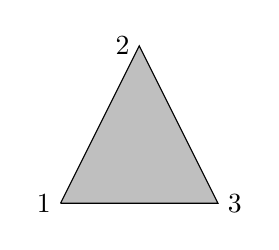
\begin{tikzpicture}
\draw [fill=gray!50] ((0,0) node[anchor = east]{1} -- (1,2) node[anchor = east]{2} -- (2,0) node[anchor = west]{3}-- (0,0);
\end{tikzpicture}
\end{frame}

\frame{\frametitle{Simplicial Complexes}
\begin{mydef}
A simplicial complex $\Delta$ on $[n] := \{1,2,\dots ,n\}$ is a finite set of simplices satisfying the following condition:
\begin{itemize}
\item For all simplices $A\in\Delta$ with $\alpha$ being a face of $A$, we have $\alpha\in\Delta$
\end{itemize}
\end{mydef}
}

\section{Boundary Functions}

\frame{\frametitle{Augmented Chain Complex}
\begin{equation*}
0\to k^{F_{n-1}(\Delta)}\overset{\partial_{n-1}}{\to}\dots\overset{\partial_{i+1}}{\to} k^{F_{i}(\Delta)}\overset{\partial_{i}}{\to}k^{F_{i-1}(\Delta)}\overset{\partial_{i-1}}{\to}\dots\overset{\partial_{0}}{\to} k^{F_{-1}(\Delta)}\to 0.
\end{equation*}\pause
\begin{mydef}[Boundary function]
For $\sigma\in F_i(\Delta)$, where $e_\sigma\in k^{F_i(\Delta)}$ is the corresponding basis vector, let $\partial_i: k^{F_i(\Delta)} \to k^{F_{i-1}(\Delta)}$ be given by 
\begin{equation*}
\partial_i(e_\sigma):=
\begin{cases}
\sum_{j\in\sigma}\textnormal{sign}(j,\sigma)e_{\sigma\setminus j} & \textnormal{ if } i=0,1,\dots,n-1 \\
0 & \textnormal{ otherwise}
\end{cases}
\end{equation*}
where $\textnormal{sign}(j,\sigma) = (-1)^{\textnormal{index}(j)-1}$.
\end{mydef}
}

\begin{frame}
\frametitle{$\partial_{i}\circ \partial_{i+1}=0$}
\pause
\begin{itemize}
\item Note that:
\begin{equation*}
0\circ\partial_{i+1}=0 \qquad \text{ and } \qquad \partial_i\circ 0 = 0.
\end{equation*} \pause
\item
Let $i=0,1,\dots,n-2$. For $\sigma\in F_{i+1}(\Delta)$ we have
\begin{equation*}
\partial_i(\partial_{i+1}(e_\sigma))=\sum_{j\in\sigma}\textnormal{sign}(j,\sigma)\sum_{k\in\sigma\setminus j}\textnormal{sign}\left(k,\sigma\setminus j\right)e_{(\sigma\setminus j)\setminus k}
\end{equation*}
by linearity of the $\partial_i$'s \pause
\item 
\begin{equation*}
=\sum_{\{j,k\}\in\sigma}\left(\textnormal{sign}(j,\sigma)\textnormal{sign}(k,\sigma\setminus j) + \textnormal{sign}(k,\sigma)\textnormal{sign}(j,\sigma\setminus k)\right)e_{\sigma\setminus\{j,k\}} 
\end{equation*}
\end{itemize}
\end{frame}

\begin{frame}
\frametitle{$\partial_{i}\circ \partial_{i+1}=0$}
\begin{itemize}
\item Assume: $\dots a \dots b \dots$
\item Then we have:
\begin{align*}
\textnormal{sign}(a,\sigma)\textnormal{sign}(b,\sigma\setminus a) &= (-1)^{\textnormal{index}(a)-1}(-1)^{(\textnormal{index}(b)-1)-1}\\
&= (-1)^{\textnormal{index}(a)-1}(-1)^{\textnormal{index}(b)-1}(-1)^{-1}\\
\textnormal{sign}(b,\sigma)\textnormal{sign}(a,\sigma\setminus b) &= (-1)^{\textnormal{index}(b)-1}(-1)^{\textnormal{index}(a)-1}\\
\end{align*} \pause
\item Which results in:
\begin{equation*}
\textnormal{sign}(j,\sigma)\textnormal{sign}(k,\sigma\setminus j) + \textnormal{sign}(k,\sigma)\textnormal{sign}(j,\sigma\setminus k) = 0
\end{equation*}\pause
\item Leading to:
\begin{equation*}
\partial_i(\partial_{i+1}(e_\sigma))=\sum_{\{j,k\}\in\sigma}0\cdot e_{\sigma\setminus\{j,k\}}
\end{equation*}
\end{itemize}
\end{frame}

\section{Homology Groups}
\begin{frame}
\frametitle{The $i$'th Reduced Homology}
\begin{equation*}
\bar{H}_i(\Delta;k):=\ker(\partial_i)/\im(\partial_{i+1}).
\end{equation*}

The $i$'th Betti number:
\begin{equation*}
H_i = \dim(\ker(\partial_i))-\dim(\im(\partial_{i+1})).
\end{equation*}
\end{frame}

\section{Betti}
\begin{frame}[fragile]
\frametitle{Betti}
\begin{lstlisting}[numbers=left]
def betti(d,maximal_faces)
    find the faces of the simplex 
    sort the faces into lengths
    for i in range(d+1) # to include bound_-1
        caluculate boundary matrix bound_i
        calculate dimensions of image and kernel of bound_i
    for i in range(d+2):
        H[i] = dim_ker_i - dim_im_i+1 # where dimensions are 0 if not calculated
    return H
\end{lstlisting}
\end{frame}

\begin{frame}[fragile]
\frametitle{Old Way of Finding Faces}
\begin{lstlisting}[numbers=left]
def prepare(simplicial_complex):
    combinations = simplicial_complex
    for maximal_face in simplicial_complex:
        for l in range(1,len(maximal_face)):
            combinations = combinations + combinations of vertices in maximal_face of length l
    combinations = list(set(combinations))
    return combinations
\end{lstlisting}
\end{frame}

\begin{frame}[fragile]
\frametitle{Finding faces}
\begin{lstlisting}[numbers=left]
def prepare(simplicial_complex)
    combinations = set([])
    for maximal_face in simplicial_complex:
    	sort maximal_face
        for i in range(len(maximal_face)):
            combinations.update(combinations of vertices in maximal_face of length i)
    return combinations    
\end{lstlisting}
\end{frame}

\begin{frame}[fragile]
\frametitle{Old Gaussian Elimination}
\begin{lstlisting}
def elimination(bound_i)
   i,j = 0,0
   while j < number of columns and i < number of rows:
       if bound_i[i,j]==0:
            find the first row, k, such that bound_i[k,j]!=0 and swap row i and k
            if there is no k
                j += 1
                continue
\end{lstlisting}
\end{frame}
\begin{frame}[fragile]
\frametitle{Old Gaussian Elimination - Continued}
\begin{lstlisting}
        scale row i such that bound_i[i,j]==1
        for L in range(number of rows):
            if L != i:
                n = bound_i[L,j]
                subtract row r from row L, n times
        i += 1
        j += 1
    return bound_i
\end{lstlisting}
\end{frame}

\begin{frame}[fragile]
\frametitle{Gaussian Elimination}
\begin{lstlisting}[numbers=left]
def elimination(bound_i)
   r,c = 0,0
   while c < number of columns and r < number of rows:
       nonzero = the nonzero row indices in [r:] of column c
       if len(nonzero) == 0:
           c += 1
           continue
\end{lstlisting}
\end{frame}

\begin{frame}[fragile]
\frametitle{Gaussian Elimination - Continued}
\begin{lstlisting}[numbers=left]
       if nonzero[0]!=r:
           swap the row of r with the row of nonzero
       pivot = bound_i[r,c]
       for L in nonzero[1:]:
           temp = bound_i[L,c]
           scale row L by pivot
           subtract row r from row L, temp times
       r += 1
       c += 1
   return bound_i
\end{lstlisting}
\end{frame}

\begin{frame}[fragile]
\frametitle{Creating Boundary Matrices}
\begin{lstlisting}[numbers=left]
def boundary(a,b):
    numrow = len(b)
    numcol = len(a)
    if numrow == 0: # if it is bound_0 being calculated
        B = matrix with 1 row and numcol columns consisting of 1s
    else:
        initialise B to a numrow*numcol matrix of 0s 
        for sigma in a:
            for j in sigma:
                i = index of sigma\j in b
                k = index of sigma in a
                B[i,k] = (-1)**(index of j in sigma) 
    return B
\end{lstlisting}
\end{frame}

\section{Datasets}
\begin{frame}
\frametitle{Datasets}
\begin{figure}
\center
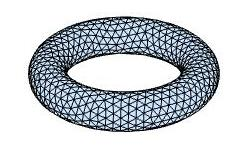
\includegraphics[scale=0.5]{torus.jpg}
\caption{Torus: Betti vector = $[0,0,2,1,0]$}
\end{figure}
\end{frame}

\begin{frame}
\frametitle{Datasets}
\begin{figure}
\center
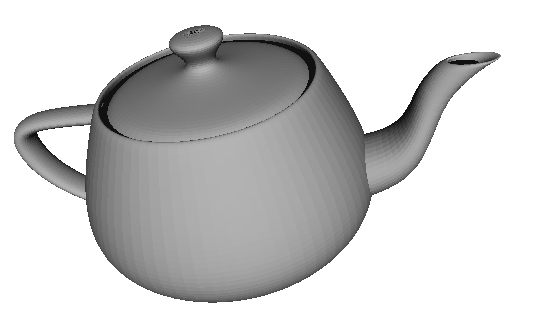
\includegraphics[scale=0.5]{teapot00.png}
\caption{Teapot: Betti vector = $[0,3,38,0,0]$}
\end{figure}
\end{frame}

\begin{frame}
\frametitle{Datasets - New Result}
\begin{figure}
\center
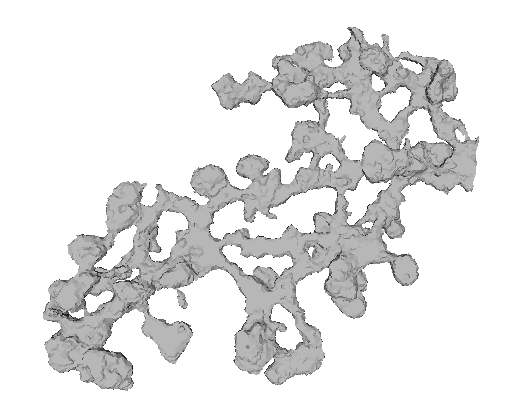
\includegraphics[scale=0.5]{testmesh00.png}
\caption{Biologic mesh: Betti vector = $[0,40,50,4,0]$}
\end{figure}
\end{frame}

\section{Conclusion}
\begin{frame}
\frametitle{Conclusion}
\begin{itemize}
\item Doesn't calculate the correct Betti vectors for graphics meshes,
\item but calculates the correct Betti vectors for simplicial complexes.
\item Not a problem when expanding to persistent homology
\item Is a limitation to the usability of the current version.
\end{itemize}
\end{frame}
\end{document}